\documentclass[twoside,11pt]{article}

% Any additional packages needed should be included after jmlr2e.
% Note that jmlr2e.sty includes epsfig, amssymb, natbib and graphicx,
% and defines many common macros, such as 'proof' and 'example'.
%
% It also sets the bibliographystyle to plainnat; for more information on
% natbib citation styles, see the natbib documentation, a copy of which
% is archived at http://www.jmlr.org/format/natbib.pdf

\usepackage{jmlr2e}
% Definitions of handy macros can go here
\usepackage{subfig}
\usepackage[skip=1em, indent=0pt]{parskip}
\usepackage{graphicx}
\usepackage{amsmath}
\graphicspath{ {./images/} }
\newcommand{\dataset}{{\cal D}}
\newcommand{\fracpartial}[2]{\frac{\partial #1}{\partial  #2}}

% Heading arguments are {volume}{year}{pages}{submitted}{published}{author-full-names}

% \jmlrheading{1}{2000}{1-48}{4/00}{10/00}{Marina Meil\u{a} and Michael I. Jordan}

% Short headings should be running head and authors last names

% \firstpageno{1}

\begin{document}
\title{COMP 424 Final Project Game: \textit{Colosseum Survival!}}
\ShortHeadings{Final project COMP 424, McGill University}{}
\author{Team Name: NafiZimu\\\\Team Members: \\Zimu Su (\texttt{zimu.su@mail.mcgill.ca}) \\Nafiz Islam (\texttt{nafiz.islam@mail.mcgill.ca})\\\\Due Date: April 8th, 2022, 11:59PM EST}

\maketitle

\section{Introduction}

Our agent is a Python module named \texttt{student\_agent.py} that consists of classes called \texttt{MCTSNode} and \texttt{StudentAgent}.

\subsection{\texttt{StudentAgent}}

\texttt{StudentAgent} is the entry point of the module for the \textit{Colosseum Survival!} game.
It consists of the \texttt{\_\_init\_\_()} method to construct the agent, helper functions, global variables, and a \texttt{step()} method.

\texttt{\_\_init\_\_()} initializes variables including \texttt{self.is\_first\_round} which is \texttt{True} if the current turn is the first turn.

The \texttt{step()} method is one of the public interface for the \textit{Colosseum Survival!} game to make a decision for a single turn.
The method sets \texttt{StudentAgent.end\_time} to the time when the MCTS should stop searching, calls \texttt{StudentAgent.mcts()}, and then returns the most optimal next position and direction discovered.

The \texttt{StudentAgent.bfs()} is a static method that performs Breadth-First Search.
It returns a generator that returns a sequence of \texttt{(number of steps, point)} where the points are legally accessible from the starting point within the maximum step.
If given the adversary's position, it will not visit the adversary's position.
This function is used to find all the legally accessible points for the player at the starting point.

The \texttt{StudentAgent.greedy\_search()} method is a static method that performs a greedy search.
It is greedy because it uses min-heap to prioritize points that are closest to the adversary's point in terms of Manhattan distance.
It also cannot pass through walls, but it ignores the maximum step.
This function serves two purpose: to determine whether both players are on the same region, or to return all the points that are within the same region as the starting point.
The purpose of making the function greedy is to stop calculating the score of a chessboard as soon as it is discovered that both players are still in the same region.

The \texttt{StudentAgent.game\_score()} method is a static method that calculates the score of the chessboard.
It returns a \texttt{tuple} where the first value is score of the first player, and the second value is the scores of the second player;
otherwise it returns \texttt{None} if both players are on the same region.
The method uses \texttt{greedy\_search()} to not only explore the region of the players and calculate their score, but also to determine if both players are on the same region much sooner.

The \texttt{StudentAgent.set\_wall()} method is a static method to set the value of a wall in a chessboard.
The method serves two purpose: to conveniently set a wall at opposite sides, and to return \texttt{True} if the wall placed is connected to other walls at both ends of the wall.
The purpose of the latter is to reduce the number of calls to \texttt{StudentAgent.game\_score()} in a Monte-Carlo method;
the assumption is that if both ends are not connected, then no new region is created, so the score would be the exact same as previous turn.

The \texttt{StudentAgent.mcts()} method is a static method that performs Monte-Carlo Tree Search using \texttt{MCTSNode} until the time limit.
After the time limit is reached, it will return the most optimal next position and direction discovered.

\subsection{\texttt{MCTSNode}}

\texttt{MCTSNode} represents a node in a Monte-Carlo Tree Search.
It could either be the root of the tree, or the children.
It consists of methods such as \texttt{\_\_init\_\_()}, \texttt{tree\_policy()}, \texttt{back\_propagation()}, \texttt{best\_child()} and \texttt{monte\_carlo\_method()}.

\texttt{\_\_init\_\_()} not only initializes fields but also performs default policy.
The purpose of performing default policy is to calculate the initial "win rate" of a node and to determine if the node can no longer be expanded.
This allows the tree policy to expand other nodes that are not finished.

\texttt{tree\_policy()} performs the tree policy of MCTS to update the score of the nodes along the most promising nodes.

\texttt{back\_propagation()} performs the back propagation to update the score of predecessors during a default policy of MCTS.

\texttt{best\_child()} returns the best direct child of an \texttt{MCTSNode}.
If the \texttt{greedy} argument is \texttt{True}, then it will pick the child with the highest win/round ratio;
otherwise, it will calculate the Upper Confidence Tree value with a scaling constant of \(\sqrt{2}\) to maintain balance between exploration and exploitation.
\texttt{greedy} is \texttt{False} when performing default policy, and \texttt{True} when picking the best next position and direction at the end of MCTS.

\texttt{monte\_carlo\_method()} performs a single Monte-Carlo method and returns a tuple which contains the score of the simulation.

There have been some consistent strategies we have applied to minimize overheads of simulating multiple games with default policy, \texttt{tree\_policy()} and \texttt{monte\_carlo\_method()}.
For example, we would modify the original copy of the chessboard and then undo the changes to avoid overhead related to copying large data.
We also perform iteration instead of recursion to avoid stack overflow, and some overheads related to managing call stack.

\section{Theory}
The basic idea we used for our implementation is the Monte Carlo Tree Search (MCTS) method.
By using Monte Carlo Method (MCM) inside MCTS, our agent could use the results from random simulations to quickly obtain a reasonable estimation of the win rate of each of its options.
Then, by combining these estimations and creating an Upper Confidence Tree (UCT), our agent can quickly grasp an idea of which option should it take for its next move.
During the entire allowed time, our agent keeps performing MCTS to reinforce its guesses and expand the UCT.
Once the allowed time is about to end, it validates the possible steps it could take, and greedily selects a final decision which could maximize its win rate.
As the game progress, the number of options our agent have reduces, which makes MCTS able to create a taller UCT in the given time. 
Since the deeper the UCT, the more simulations the agent gets to do, the agent's estimation becomes more accurate as the game progresses closer to the end.

The number of possible states (position and wall at that position) at each turn could be calculated using the following formula.
For simplicity of calculation, we ignore the walls that are existing in the following formula.
K stands for the max number of steps the agent is allowed to take.

\begin{equation}
	4\times\left(1 + 4\sum_{n=1}^{K}{n}\right)
\end{equation}

\begin{table}[!ht]
	\centering
	\begin{tabular}{|l|l|l|l|l|}
		\hline
		K & 2 & 3 & 4 & 5  \\ \hline
		\# of branches & 52 & 100 & 164 & 244  \\ \hline
	\end{tabular}
\end{table}

As we can see in the table above, the branching factor of the search tree gets large quickly.
Thus, we incorporated more randomness to the MCTS we learned in class to reduce the size of the search tree. 
Instead of going through all the possible options each time, our agent only explore on roughly half of the options. 
By doing so, the agent could get to a deeper depth with exploitation, which makes its guesses less of a product of luck and more of a reliable estimation.

\section{Analysis}
As mentioned in the theory section, our agent mainly follows MCTS method. 
We made some changes to the normal MCTS so it favours exploitation over exploration. 
And, we gave it a internal "time limit", so it always finishes its decision within the allowed time.

\subsection{Advantages}
One of the main advantages of our agent is that it is unlikely to take more than the allowed time to select a move. 
In other words, we configured our agent so that it has a low "misplay rate".
(This is because whenever the agent goes overtime, it will be forced to choose a random move.)
In order to do so we have to sacrifice some of the exploration options. 
This means that our agent might miss some really good opportunities to close the game off. 
But more generally speaking, this could make our agent always walk on a path that favours our win a little bit more, and we believe this trade off between risk and consistency is worth it.

In addition, since our implementation did not have any built-in static variable (except the time constraints), our agent could be used in maps that are larger than the 10x10 limit. 
The performance of the agent will decrease as the size of the map gets larger, and when facing a very large map, the agent might not be able to return an answer in 2 seconds.
But with some simple tweaking of variables, we believe that the agent should be able to work in a larger scale.

\subsection{Disadvantages}
The biggest issue with our agent comes from the possibility of it missing some winning steps.
Since we are not exploring all the possible steps, and we are randomly choosing the steps that we want to evaluate, the chance of our agent misses its opportunities is fairly high.
To solve this issue, we implemented a simple mechanism where if the number of all possible steps is small enough, our agent will evaluates all of them.
This mechanism gives our agent a higher chance of "noticing" the winning moves when the chessboard is filled with walls, so it helps our agent a lot during late game. 
However, this implementation doesn't solve all the issues. 
The agent still could miss some good opportunities during the early stage of a game.

The fact that it isn't playing optimally in the early stage isn't ideal, but it is not unacceptable.
Our agent will become a lot more "deadly" during the late game, and it will not miss any opportunity by then, thus we think it is acceptable to miss some win potentials and trade it for consistency. 
As mentioned previously, our agent will always do a move that favours its win.
We believe by accumulating this advantage, our agent could slowly but steadily reach the winning state.

\subsection{Failure Modes}
The most common failure case is that in some early state, the agent missed the chance to finish the opponent, then it proceeded to move in to a position that it thought would be beneficial, but actually let the opponent escape.

The following images shows one occurrence of this failure:\\
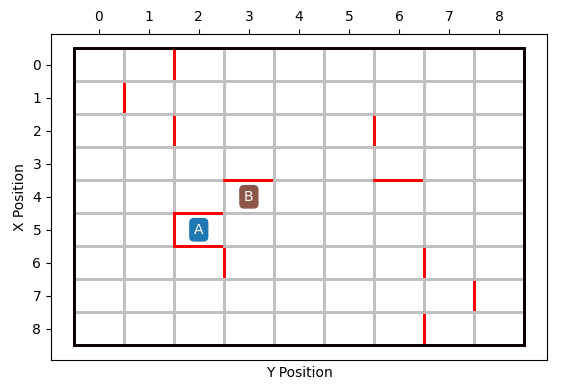
\includegraphics[width=0.5\textwidth]{b_skip_1.png}
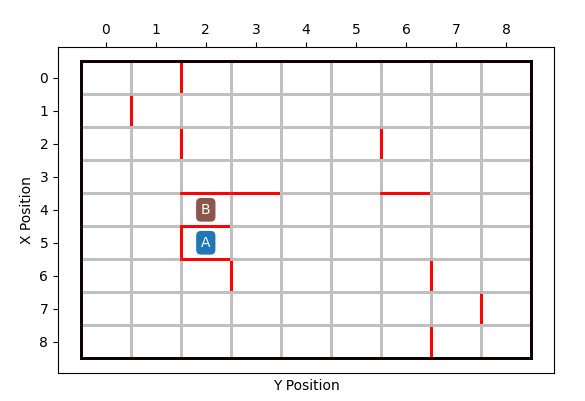
\includegraphics[width=0.5\textwidth]{b_skip_2.png}

As explained previously, this failure occurs because of the incompleteness of the options of our agent.
As of our current implementation, there is no way to completely remove this failure without harming the searching time.

\section{Other Approach}
During the brainstorming part of the project, we thought about multiple ideas such as Minimax, Monte-Carlo Tree Search and \(\alpha\)-\(\beta\) Pruning.
We figured that \(\alpha\)-\(\beta\) Pruning is better than Minimax in general, there is no need to consider Minimax, which left us with two options: Monte-Carlo Tree Search and \(\alpha\)-\(\beta\) Pruning.

\subsection*{\(\alpha\)-\(\beta\) Cutoff Pruning}
We initially thought about using \(\alpha\)-\(\beta\) Pruning in our solution.
Since \(\alpha\)-\(\beta\) Pruning requires our agent to go search until the end state of the game, we thought it would be too expensive both computationally, and time-wise.
Therefore, we incorporated MCM with \(\alpha\)-\(\beta\) Pruning to create our modified version of \(\alpha\)-\(\beta\) Pruning, so that it could return the best moves to choose based on the simulated results, similar to the Minimax Cutoff algorithm we discussed in class.

We made a prototype of the \(\alpha\)-\(\beta\) Cutoff Pruning in the early version of the agent. 
It seemed to be working and it was selecting rational moves most of the time. 
However, the time it took to compute a move varies drastically depending on the size of the board. 
At a board size of 4, the agent is able to decide on a move almost instantly, but when the board size exceed 7, every decision of the agent took more than 30 seconds.
We thought this is unacceptable because it doesn't fall in the time limit of the tournament.
Therefore we tried to adjust the agent by adjusting the number of samples MCM does and number of possible next steps \(\alpha\)-\(\beta\) Cutoff Pruning considers.
However, nothing seemed to improve the performance of our agent to an acceptable level.
Thus, we decided to drop \(\alpha\)-\(\beta\) Cutoff Pruning, and went with MCTS.

\section{Possible Improvement}

There are a few possible improvements that can be made in the Monte-Carlo Tree Search.
The simplest improvement that can be made is to prioritize adjacent state spaces that would add a wall that is connected to another wall.
This would maximize the value of the children nodes since a human player would intuitively place a wall that is connected to another wall to quickly create a closed region.
However, we should still include other state spaces that do not connect walls;
for example, placing an unconnected wall can prevent the adversary from winning by forcing it to take extra step.

Another possible optimization is to reuse an existing Monte-Carlo tree search.
This would allow us to take advantage of the 30 seconds in the first round to build a large search tree and then reuse a subsection of the tree to avoid rebuilding an entire tree for the subsequent rounds.
Nonetheless, this might not be effective because the branching factor of the game is very large, so the likelihood that the adversary will visit an already expanded node might be low. 

% \vskip 0.2in
% \bibliography{sample}

\end{document}